This section described the implementation aspects of the front end of the system. As the front end is primaraly responsible
with the i/o of the system it is unlikely to be a bottleneck in the performance of the system, as a result little effort
has been expended into optimising the front-end.

\subsection{Scene Input (1.5 pages)}
The scene input is read into a data structure that is passed to the back-end, this structure is implemented as a C struct
containing a list of all objects in the scene, a camera definition that defines how the eye rays are created.

Mesh input to the scene allows for each of the meshes to have matrix operations applied to them, these trasformations
are applied at the construction of the mesh prior to creating the kdtree of the mesh.

\subsection{Command Line (0.1 pages)}
Users are able to input command line arguments to the system, these are received by C programs in the input parameters of
the main function, these input parameters need to be parsed and stored, this is performed by simply scanning over each
option in the argv list to find a valid option or pair of options in the case of a user inputed value for the option
i.e. width of the output image.

\begin{figure}
\texttt{./raytracer -w 1000 -h 1000 -i ./data/scenes/cornell\_box.scene}
\caption{Example command line.}
\end{figure}

\subsection{Global Configuration}
Once the configuration of the scene has been read and processed the data containing the configuration will not change for
the lifetime of the program, as a result the global configuration is available in the system through a global variable, while
it is generally advised whene developing software that global variable should be avoided an implementation that passed the
configuration would require that a pointer to a configuration structure be passed, this amounts to having the same result
as a global variable whilst reducing the clarity of the code.

\begin{figure}
\centering
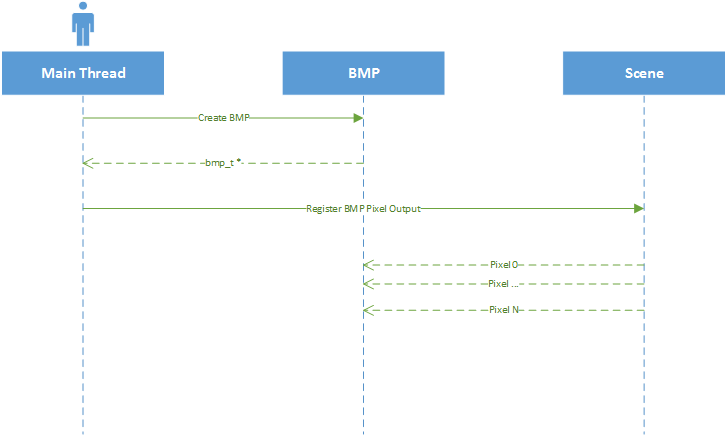
\includegraphics[width=\textwidth]{./images/pixel_update_sequence.png}
\caption{Sequence for pixel update}
\end{figure}

\subsection{Common Pixel Update Interface}
In order to make integration of the system as simple as possible we have created an interface that will encapsulate the data
that is passed from the backend to the front-end to be presentend to the user, this facilitated the decoupling of the front
and back-end. Two modules have been created that use the interface to demonstrate the useage of the interface, these are
desctibed below. The common pixel output is implemented by registering output from the system through a function pointer,
this pointer will be called whenever a pixel is received from the back-end.

\subsubsection{Image Output (0.5 pages)}

The systems output image type is BMP (extension .bmp) this image format was chosen as it is a simple image format, there are
several variants of BMP each with its own header definition the version of BMP that is implemented is the OS/2 bitmap this is
one of the more simple variants with a fixed size header that specified few options. The implementation of the BMP output can
be found in \texttt{bmp.h/c}. If supported on the platform the system is also capable of outputing images in PNG file format,
this is acheived by using libPNG, there are advantages to outputing to this format, foremost is that the image size of an
image output to PNG is significantally smaller than that outputed by BMP.

\todo{maybe include size graph (might not be relivant though)}

\subsubsection{GUI (0.5 pages)}

The User Interface That is included in the system is designed to allow instant feedback to the user of the render, this can be
useful in the case of errors that can be identified early in what may be a costly render, the interface is rather simple
providing only a surface that displays the current state of the render.

I have decided to use SDL library to provide the interface to the operating system window system and OpenGL to perform the 
drawing of the pixels to the screen.

SDL (Simple Direct media Library) is a library that allows for cross platform applications to be written that include
drawable surfaces, OpenGL support and user input, SDL is written in C and provides a library API for C.

In order to retain responsivness of the GUI while rendering it is desirable to run the GUI on a seperate thread, the GUI
should also only redraw the screen when a pixel has updated its colour, this is to reduce the amount of processing that
the GUI is performing that could be used to create images, on the other had the GUI should respond to events that are pushed
to its internal event queue such as key presses and window system events.

